\chapter{Spherical harmonics}\label{app:SH}
The (complex)
spherical harmonic function of degree $n$ and order $m$\\ ($n\in\mathbb{N}_0,\ m\in\mathbb{Z}, 0\leq \abs{m} \leq n$) 
is defined as
\begin{equation}\label{eq:Ynm}
\nomenclature[a]{$\Y{n}{m}$}{spherical harmonic function of degree $n$ and order $m$\nomrefeq}
    \Y{n}{m}(\bomega) = \Y{n}{m}(\polar,\azimuthal) = 
    \sqrt{\frac{2n+1}{4\pi}\frac{(n-m)!}{(n+m)!}} \P{n}{m}(\cos\polar)e^{i m \azimuthal},
\end{equation}
or, if we denote $\mu \equiv \cos\polar$,
$$
	\Y{n}{m}(\mu,\azimuthal) = \sqrt{\frac{2n+1}{4\pi}\frac{(n-m)!}{(n+m)!}} \P{n}{m}(\mu)e^{i m \azimuthal},
$$
where
\begin{equation}\label{eq:associated_Pn}
    \nomenclature[a]{$\P{n}{m}(\mu)$}{associated Legendre polynomial of degree $n$ and order $m$\nomrefeq} 
    \P{n}{m}(\mu) = 
    \begin{cases} 
    	(-1)^m\sqrt{(1-\mu^2)^m}\ \der[m]{\P{n}{}(\mu)}{\mu} & \mbox{if } \hphantom{-}\,0 \leq m \leq n,\\[.5em]
    \displaystyle (-1)^{-m}\frac{(n+m)!}{(n-m)!}\P{n}{-m}(\mu) & \mbox{if } -n \leq m < 0 
    \end{cases}
\end{equation}
are the \textit{associated Legendre functions}. Note that ordinary Legendre polynomials are recovered for $m = 0$:
\begin{equation*}
\begin{gathered}
	\P{0}{}(\mu) = 1,\quad \P{1}{}(\mu) = \mu,\quad \P{2}{}(\mu) = \frac12(3\mu^2 - 1),
\quad \P{3}{}(\mu) = \frac12(5\mu^3 - 3\mu),\\
 	(2k + 1)\mu\P{k}(\mu) = (k+1)\P{k+1}(\mu) + k\P{k-1}(\mu)
\end{gathered}
\end{equation*}

The complex spherical harmonics form a closed orthonormal system on $\Lp{2}(\Sphere)$ with respect to the
standard inner product $$
(\psi, \varphi)_{\Lp[2](\Sphere)} = \intA{\psi(\bomega) {\overline\varphi(\bomega)}}
$$
(where the overline denotes complex conjugation), that is
$$
\begin{aligned}
\intA{\Y{n}{m}(\bomega)\Yc{n}{m}(\bomega)} &=
\int_{0}^{2\pi}\d{\azimuthal}\int_{0}^{\pi}\sin\polar\d{\polar}  
\Y{n}{m}(\polar,\azimuthal)\Yc{l'}{m'}(\polar,\azimuthal)\\[.25em]
& = \int_{0}^{2\pi}\d{\azimuthal}\int_{-1}^{1}\d{\mu}
\Y{n}{m}(\mu,\azimuthal)\Yc{l'}{m'}(\mu,\azimuthal) = \kron{m}{m'}\kron{n}{l'}
\end{aligned}
$$
where $\kron{i}{j} = 1$ if $i = j$ and $\kron{i}{j} = 0$ otherwise (Kronecker delta symbol). They also satisfy the
following \textit{addition theorem}, which allows to express the value of Legendre polynomial of degree $k$ at $\mu_0 =
\bomega\cdot\bomega'$ as a dot product of vectors with values of the $2k+1$ spherical harmonics at $\bomega$ and
$\bomega'$, respectively:
\begin{align}
\P{k}(\mu_0)
&=P_k(\mu) P_k(\mu')+2 \sum _{m = 1}^k \frac{(k-m)!}{(k+m)!} \cos \bigl(m(\azimuthal - \azimuthal')\bigr) P_k^m(\mu) P_k^m(\mu')\nonumber\\
&=\frac{4\pi}{2k+1}\suma[m]{-k}{k}\Y{k}{m}(\polar,\azimuthal)\Yc{k}{m}(\polar',\azimuthal'),
\label{eq:additionThm}
\end{align}
Note that this greatly simplifies integrals of type
$$
\intA{P_k(\bomega\cdot\bomega')f(\bomega')}
$$
(as in \alert{ref}), because of the complicated form of $\bomega\cdot\bomega'$:
$$
\begin{aligned}
	\mu_0 = \bomega'\cdot\bomega 
&= \lvect{\sint'\cosp',\sint'\sinp',\cost'} \cdot 
	\lvec{\sint\cosp,\sint\sinp,\cost}\\
& = \mu'\mu + \sqrt{(1-\mu'^2)(1-\mu^2)}\cos(\azimuthal' - \azimuthal),
\end{aligned}
$$
where $\mu = \cost$\nomenclature[g]{$\mu$}{cosine of the polar component of the direction vector $\bomega$} is the
 cosine of the polar component of the direction vector $\bomega$ (see \fref{fig:scatter}).
\begin{figure}[!hbt]
    \centering
    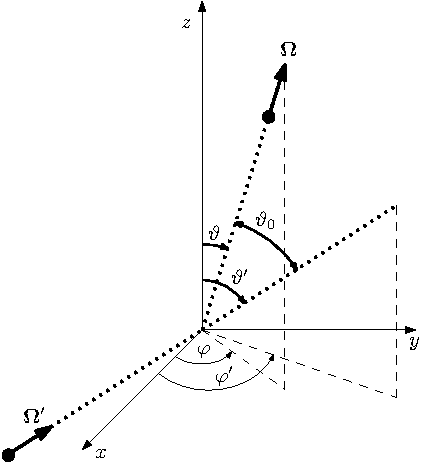
\includegraphics[scale=1.65]{scattering.eps}
    \caption[Scattering]{Geometry of scattering}
    \label{fig:scatter}
\end{figure}

A real basis of spherical harmonics can be obtained from complex linear combination of the original basis and can be
written in the following form:
\begin{gather*}
    \y{n}{m}(\polar,\azimuthal) = 
    \begin{cases}
    	\sqrt{2} C_n^m \P{n}{m}(\cos\polar)\cos(m \azimuthal) = \mathrm{Re}\,\Y{n}{m}(\polar,\azimuthal) & m > 0,\\[.2em]
    	C_n^0 \P{n}{0}(\cos\polar) = \Y{n}{0}(\polar,\azimuthal) & m = 0,\\[.2em]
    	\sqrt{2} C_n^{-m} \P{n}{-m}(\cos\polar)\sin(-m \azimuthal) = \mathrm{Im}\,\Y{n}{-m}(\polar,\azimuthal) & m < 0,
    \end{cases}\\[.5em]
    C_n^m = \sqrt{\frac{2n+1}{4\pi}\frac{(n-m)!}{(n+m)!}}.   
\end{gather*}
Functions $\y{n}{m}$ are usually called \textit{tesseral spherical harmonics of degree $n$ and order $m$} (sometimes the
case $n = m$ is distinguished as \textit{sectorial spherical harmonics}). Linear combination of tesseral spherical
harmonics of degree $n$ produces a \textit{surface spherical harmonic of degree $n$}:
\begin{equation*}
\begin{multlined}
    \mathcal{Y}_n(\bomega) = \mathcal{Y}_n(\polar,\azimuthal) = \\A_0 P_n(\cos\polar) + \suma[m]{1}{n}\left[ A_m
    \cos(m\azimuthal)\P{n}{m}(\cos\polar) + B_m \sin(m\azimuthal)\P{n}{m}(\cos\polar)\right]
  \end{multlined}
  \end{equation*}
Surface spherical harmonics are formally defined as restrictions of homogeneous harmonic polynomials of degree $n$ to
unit sphere $\Sphere$ (\cite[Art. 110]{Byerly}, \cite[Def. 3.22]{Schreiner}).

\newpage
\begin{sidewaysfigure}
	\centering
		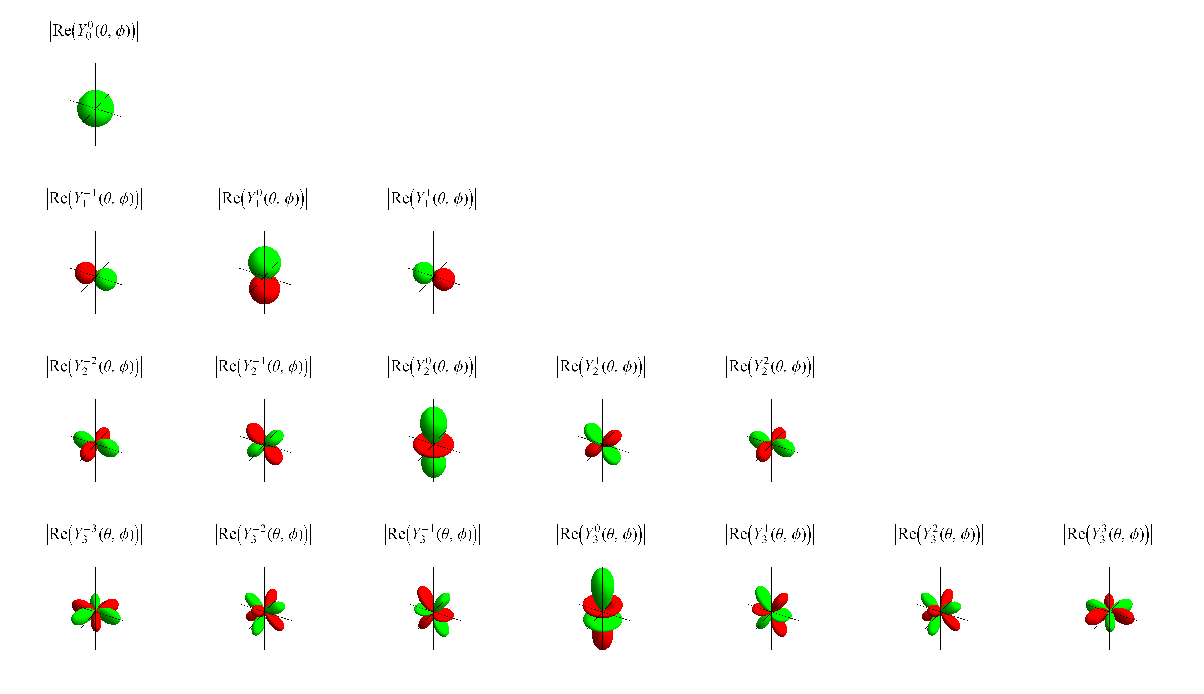
\includegraphics[scale=1.2]{pic/sh.eps}
		\caption[Spherical harmonics]{Spherical harmonics up to $3^{\mbox{rd}}$ degree, plotted in spherical coordinates 
		as specified in the labels above the graphs and colored green if $\mathrm{Re}\,\Y{n}{m} \geq 0$ and red
		otherwise (picture generated by Mathematica 7.0).}%
	\label{fig:SH} 
\end{sidewaysfigure}



